%
% Niniejszy plik stanowi przykład formatowania pracy magisterskiej na
% Wydziale MIM UW.  Szkielet użytych poleceń można wykorzystywać do
% woli, np. formatujac wlasna prace.
%
% Zawartosc merytoryczna stanowi oryginalnosiagniecie
% naukowosciowe Marcina Wolinskiego.  Wszelkie prawa zastrzeżone.
%
% Copyright (c) 2001 by Marcin Woliński <M.Wolinski@gust.org.pl>
% Poprawki spowodowane zmianami przepisów - Marcin Szczuka, 1.10.2004
% Poprawki spowodowane zmianami przepisow i ujednolicenie 
% - Seweryn Karłowicz, 05.05.2006
% Dodanie wielu autorów i tłumaczenia na angielski - Kuba Pochrybniak, 29.11.2016

% dodaj opcję [licencjacka] dla pracy licencjackiej
% dodaj opcję [en] dla wersji angielskiej (mogą być obie: [licencjacka,en])
\documentclass[licencjacka,en]{pracamgr}

\usepackage{graphicx} %package to manage images
\graphicspath{ {./images/} }

\usepackage[rightcaption]{sidecap}

\usepackage{wrapfig}

% Dane magistranta:
% \autor{Adam Deryło, Adrian Hess, Magdalena Pałkus, Michał Skwarek}{34234234}

% Dane magistrantów:
\autor{Adam Deryło}{342007}
\autori{Adrian Hess}{342013}
\autorii{Magdalena Pałkus}{231023}
\autoriii{Michał Skwarek}{777321}
%\autoriv{Autor nr Cztery}{432145}
%\autorv{Autor nr Pięć}{342011}

\title{GPU acceleration of CCSDS Rice decoding}
\titlepl{Akcerleracja GPU dekodowania CCSDS Rice}

%\tytulang{An implementation of a difference blabalizer based on the theory of $\sigma$ -- $\rho$ phetors}

%kierunek: 
% - matematyka, informacyka, ...
% - Mathematics, Computer Science, ...
\kierunek{Computer Science}

% informatyka - nie okreslamy zakresu (opcja zakomentowana)
% matematyka - zakres moze pozostac nieokreslony,
% a jesli ma byc okreslony dla pracy mgr,
% to przyjmuje jedna z wartosci:
% {metod matematycznych w finansach}
% {metod matematycznych w ubezpieczeniach}
% {matematyki stosowanej}
% {nauczania matematyki}
% Dla pracy licencjackiej mamy natomiast
% mozliwosc wpisania takiej wartosci zakresu:
% {Jednoczesnych Studiow Ekonomiczno--Matematycznych}

% \zakres{Tu wpisac, jesli trzeba, jedna z opcji podanych wyzej}

% Praca wykonana pod kierunkiem:
% (podać tytuł/stopień imię i nazwisko opiekuna
% Instytut
% ew. Wydział ew. Uczelnia (jeżeli nie MIM UW))
\opiekun{Paweł Gora\\
  Faculty of Mathematics, Informatics and Mechanics, University of Warsaw\\
  }

% miesiąc i~rok:
\date{Jan 2023}

%Podać dziedzinę wg klasyfikacji Socrates-Erasmus:
\dziedzina{ 
%11.0 Matematyka, Informatyka:\\ 
%11.1 Matematyka\\ 
% 11.2 Statystyka\\ 
11.3 Informatics, Computer Science \\ 
%11.3 Informatyka\\ 
%11.4 Sztuczna inteligencja\\ 
%11.5 Nauki aktuarialne\\
%11.9 Inne nauki matematyczne i informatyczne
}

%Klasyfikacja tematyczna wedlug AMS (matematyka) lub ACM (informatyka)
\klasyfikacja{D. Software\\
  D.1.3. Concurrent Programming\\
  I.4.2. Compression (Coding) \\ }

% Słowa kluczowe:
\keywords{CCSDS Rice coding, GPU, Compute Unified Device Architecture (CUDA)}

% Tu jest dobre miejsce na Twoje własne makra i~środowiska:
\newtheorem{defi}{Definicja}[section]

% koniec definicji

\begin{document}
\maketitle

%tu idzie streszczenie na strone poczatkowa
\begin{abstract}
	TBD
\end{abstract}

\tableofcontents
%\listoffigures
%\listoftables

\chapter*{Introduction}
\addcontentsline{toc}{chapter}{Introduction}
Data compression is a widely utilized technique for reducing the storage requirements and
transmission time for large data sets. However, when it comes to training deep learning models,
the decompression of compressed data can create a bottleneck in the machine learning pipeline, particularly
when dealing with specialized data formats such as astronomy and medicine that employ custom compression
algorithms that can be computationally expensive to decompress.One such specialized compression algorithm is RICE coding,
which is widely used in the FITS data format in astronomy. To address this bottleneck,
utilizing Graphics Processing Units (GPUs) and parallelization techniques have emerged as promising solutions
for accelerating the decompression of large data sets by leveraging the parallel processing capabilities of GPUs.
While established solutions for mainstream lossless compression algorithms like JPEG-2000 exist,
this paper aims to investigate the potential of GPU acceleration and parallelization
in enhancing the performance of RICE coding, a specialized and niche compression algorithm.


\chapter{Key terms}\label{r:pojecia}

\section{FITS}
The Flexible Image Transport System (FITS) format is a digital file format that is commonly
utilized in the field of astronomy for storing and transferring scientific data. FITS files
typically contain images, data cubes, and tables of observational data, as well as associated metadata.
One of the key characteristics of FITS is its ability to store multiple data arrays in a single file, which
allows for the efficient storage and transfer of large data sets. The FITS format is an open standard
and is supported by a wide range of software and data analysis tools. However, the FITS format is also
known for its large file size, which can present challenges when working with large data sets.
As a result, compression algorithms such as RICE compression are often applied to the data before storing in the FITS format. \\

Citing NASAs fits standard: \\
A FITS file shall be composed of the following FITS structures,
in the order listed:
\begin{itemize}
	\item Primary header and data unit (HDU).
	\item Conforming Extensions (optional).
	\item Other special records (optional, restricted).
\end{itemize}
Thus, FITS files have follwoing structure:
\begin{figure}[t]
	\centering
	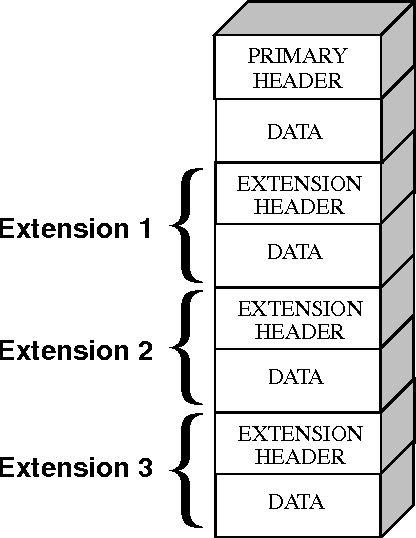
\includegraphics[scale=0.3]{fits}
\end{figure}

\newpage






\section{RICE}

\chapter{GPU acceleration of CCSDS Rice decoding algorithm}\label{r:losers}

\section{Naive approach}







\begin{thebibliography}{99}
	\addcontentsline{toc}{chapter}{Bibliography}

	\bibitem[Bea65]{beaman} Juliusz Beaman, \textit{Morbidity of the Jolly
		function}, Mathematica Absurdica, 117 (1965) 338--9.


\end{thebibliography}

\end{document}


%%% Local Variables:
%%% mode: latex
%%% TeX-master: t
%%% coding: latin-2
%%% End:
